% !TeX spellcheck = pt_BR

%%%%%%%%%%%%%%%%%%%%%%%%%%%%%%%%%%%%%%%%
% Classe do documento
%%%%%%%%%%%%%%%%%%%%%%%%%%%%%%%%%%%%%%%%

% Nós usamos a classe "unb-cic".  Deixe apenas uma das linhas
% abaixo não-comentada, dependendo se você for do bacharelado ou
% da licenciatura.

% Para tirar os comentários, é só mudar o comando para fazer nada.
\newcommand{\com}[1]{\textcolor{red}{#1}}%

\documentclass[mpca]{unb-cic}



%%%%%%%%%%%%%%%%%%%%%%%%%%%%%%%%%%%%%%%%
% Pacotes importados
%%%%%%%%%%%%%%%%%%%%%%%%%%%%%%%%%%%%%%%%

\usepackage[brazil,american]{babel}
\usepackage[T1]{fontenc}
\usepackage{indentfirst}
\usepackage{natbib}
\usepackage{xcolor,graphicx,url}
\usepackage[utf8]{inputenc}
\usepackage{amsmath,amssymb,amsthm}
\usepackage{footnote}
%\usepackage{minipage}
\usepackage{float}
\usepackage{tablefootnote} 
\usepackage{listings}
\usepackage{myglossary}


%%%%%%%%%%%%%%%%%%%%%%%%%%%%%%%%%%%%%%%%
% Cores dos links
%%%%%%%%%%%%%%%%%%%%%%%%%%%%%%%%%%%%%%%%

% Veja o arquivos cores.tex se quiser ver que outras cores estão
% pré-definidas.  Utilizando o comando \hypersetup abaixo nós
% evitamos aquelas caixas vermelhas feias em volta dos links.

%%%%%%%%%%%%%%%%%%%%%%%%%%%%%%%%%%%%%%%%
% Cores do estilo Tango
%%%%%%%%%%%%%%%%%%%%%%%%%%%%%%%%%%%%%%%%

\definecolor{LightButter}{rgb}{0.98,0.91,0.31}
\definecolor{LightOrange}{rgb}{0.98,0.68,0.24}
\definecolor{LightChocolate}{rgb}{0.91,0.72,0.43}
\definecolor{LightChameleon}{rgb}{0.54,0.88,0.20}
\definecolor{LightSkyBlue}{rgb}{0.45,0.62,0.81}
\definecolor{LightPlum}{rgb}{0.68,0.50,0.66}
\definecolor{LightScarletRed}{rgb}{0.93,0.16,0.16}
\definecolor{Butter}{rgb}{0.93,0.86,0.25}
\definecolor{Orange}{rgb}{0.96,0.47,0.00}
\definecolor{Chocolate}{rgb}{0.75,0.49,0.07}
\definecolor{Chameleon}{rgb}{0.45,0.82,0.09}
\definecolor{SkyBlue}{rgb}{0.20,0.39,0.64}
\definecolor{Plum}{rgb}{0.46,0.31,0.48}
\definecolor{ScarletRed}{rgb}{0.80,0.00,0.00}
\definecolor{DarkButter}{rgb}{0.77,0.62,0.00}
\definecolor{DarkOrange}{rgb}{0.80,0.36,0.00}
\definecolor{DarkChocolate}{rgb}{0.56,0.35,0.01}
\definecolor{DarkChameleon}{rgb}{0.30,0.60,0.02}
\definecolor{DarkSkyBlue}{rgb}{0.12,0.29,0.53}
\definecolor{DarkPlum}{rgb}{0.36,0.21,0.40}
\definecolor{DarkScarletRed}{rgb}{0.64,0.00,0.00}
\definecolor{Aluminium1}{rgb}{0.93,0.93,0.92}
\definecolor{Aluminium2}{rgb}{0.82,0.84,0.81}
\definecolor{Aluminium3}{rgb}{0.73,0.74,0.71}
\definecolor{Aluminium4}{rgb}{0.53,0.54,0.52}
\definecolor{Aluminium5}{rgb}{0.33,0.34,0.32}
\definecolor{Aluminium6}{rgb}{0.18,0.20,0.21}

\hypersetup{
  colorlinks=true,
  linkcolor=DarkScarletRed,
  citecolor=DarkScarletRed,
  filecolor=DarkScarletRed,
  urlcolor= DarkScarletRed
}



%%%%%%%%%%%%%%%%%%%%%%%%%%%%%%%%%%%%%%%%
% Informações sobre a monografia
%%%%%%%%%%%%%%%%%%%%%%%%%%%%%%%%%%%%%%%%
\title{Extensão do UnBBayes para suportar Incremental Learning de Redes Bayesianas}%

\orientador{\prof \dr Marcelo Ladeira}{CIC/UnB}
\coorientador{\prof Shou Matsumoto}{CIC/GMU}
\coordenador[a]{\prof[a] \dr[a] Coorde Nadora}{CIC/UnB}
\diamesano{07}{dezembro}{2015}%

\membrobanca{\prof[a] \dr[a] Membra da Banca}{MEC}
\membrobanca{\prof \dr Membro do Banco}{CIC/UnB}

\autor{Guilherme C.}{Torres}
\autor{Guilherme N.}{Ramos}
\CDU{004.4}

\palavraschave{Redes Bayesianas, UnBBayes, Aprendizado, Design Pattern}
\keywords{\LaTeX, scientific method}



\graphicspath{{.}{img/}}%
\newcommand{\unbcic}{\texttt{UnB-CIC}}%





%%%%%%%%%%%%%%%%%%%%%%%%%%%%%%%%%%%%%%%%
% TextoF
%%%%%%%%%%%%%%%%%%%%%%%%%%%%%%%%%%%%%%%%



\begin{document}
  \maketitle

  \begin{dedicatoria}
Citando o poeta: ``Eu dedico essa música a primeira garota que tá sentada ali na fila. Brigado!''
  \end{dedicatoria}

  \begin{agradecimentos}
Agradeço ao Prof. José Ralha, cujos esforços na versão anterior foram bem ``adaptados'' a este trabalho.
  \end{agradecimentos}

\hyphenation{au-xi-li-ar}

  \begin{resumo}
	Com o crescente interesse em aprendizado de máquina, frameworks robustos e implementações do estado da arte são uma necessidade do mundo moderno. Pensando nisso levantamos um estudo sobre o estado da arte de aprendizado no contexto de \gls{bn}, já que \glspl{bn} provêm um excelente modelo para lidar com relações causais e probabilidade bayesiana. Para tal utilizaremos o framework UnBBayes e desenvolveremos plugins para este.
  \end{resumo}
  

  \selectlanguage{american}
  \begin{abstract}
  With the growing interest in machine learning, good frameworks and state of the art implementation are a need in modern world. With this in mind we provide a study in the state of the art of \gls{bn}, since \glspl{bn} provide a great model to deal with causal relations and bayesian probability. For such we shall use UnBBayes framework and implement plugins for it.
  \end{abstract}
  \selectlanguage{brazil}
\hyphenation{a-tri-bu-tos}

  \tableofcontents
  \listoffigures
  \listoftables
  \printnoidxglossaries
\renewcommand{\appendixname}{Anexo}


  \textual
  No cotidiano do ser humano é muito comum raciocinar e tomar decisões sob condições de incerteza. Isto é tão visível e profundo para algumas pessoas que no século XVIII Bishop Butler declarou "probabilidade é o guia da vida".

Como um exemplo do quanto probabilidade é importante tome a medicina. Para um especialista médico determinar a doença de uma pessoa com base nos sintomas observados (evidências) é preciso que ele leve em conta a probabilidade daquele sintoma refletir esta ou aquela doença, pois a doença ocasiona determinado sintoma apenas com alguma probabilidade, mas não com certeza.

Podemos ainda citar vários outros exemplos, como na economia, teoria dos jogos, genética, previsão do tempo.

Pensando nisso é necessário um modelo robusto para lidar com tantas incertezas, para tanto escolhemos as \glspl{bn}.

\section{Motivação}
\gls{bn} é um modelo gráfico para relações probabilísticas dado conjunto de variáveis. Nas últimas décadas, redes Bayesianas se tornaram representações populares para codificar conhecimento incerto para sistemas especialistas \cite{heck95}. Mais recentemente, pesquisadores desenvolveram métodos de aprendizagem de redes Bayesianas a partir de dados. As técnicas desenvolvidas são relativamente novas e ainda em evolução, mas eles têm se mostrado muito eficientes para alguns problemas de análise de dados.

Existem diversos representações possíveis para analise de dados, entre elas, decision tres, e redes neurais artificiais; e outras tantas como estimação de densidade, classificação, regressão e clusterings. Portanto o que métodos de \glspl{bn} têm a oferecer? Segundo Heckerman \cite{heck95} podemos oferecer pelo menos quatro respostas, sendo elas:

\begin{enumerate}
	\item \glspl{bn} lidam com um conjunto incompleto de dados de maneira natural.

	\item \glspl{bn} permitem aprender sobre as relações causais. Aprender sobre tais relações são importantes por pelo menos duas razões: O processo é útil quando se está tentando entender sobre um dado problema de domínio, como por exemplo, durante uma análise de dados exploratória.  E mais, conhecimento de relações causais nos permitem fazer predições na presença de intervenções. Por exemplo, um analista de mercado pode querer saber se é lucrativo aumentar o investimento em determinada propaganda para aumentar as vendas de seu produto. Para responder esta pergunta o analista pode determinar se esta propaganda é a causa para o aumento de suas vendas, e em caso afirmativo, quanto. O uso de \glspl{bn} nos ajuda a responder tal pergunta até mesmo quando não há experimentos nos efeitos de tal propaganda.
	
	\item \glspl{bn} em conjunto com técnicas estatísticas bayesianas facilitam a combinação de conhecimento de domínio e dados. Qualquer um que tenha feito uma análise do mundo real sabe a importância de conhecimento prévio ou de domínio, em especial quando os dados são poucos ou caros. Pelo fato de alguns sistemas comerciais (i.e., sistemas especialistas) podem ser construídos a partir de conhecimentos prévios. \cglspl{bn} possuem uma semântica causal que permitem conhecimentos prévios serem representados de uma forma muito simples e natural. Além disto, \glspl{bn} encapsulam tais relações causais com suas probabilidades. Consequentemente, conhecimento prévio e dados podem ser combinados com técnicas bem estudadas da estatística Bayesiana.
	
	\item Métodos Bayesianos em conjunto com \glspl{bn} e outros tipos de modelos oferecem uma forma eficiente para evitar over fitting dos dados. Como veremos, não há necessidade de excluir parte dos dados do treinamento do aprendizado da rede. Usando técnicas Bayesianas, modelos podem ser "suavizados" de tal forma que todo dado disponível pode ser usado para o treinamento.

\end{enumerate}

\section{Objetivos}
O objetivo deste trabalho é apresentar os conhecimentos adquiridos durante este semestre na disciplina de Estudos Em Inteligência Artificial com o professor Ladeira da \gls{unb}, com a colaboração do Doutorando Shou Matsumoto da \gls{gmu}, através de aulas pelo skype. E também firmar bases sólidas sobre os conhecimentos que serão necessários na concepção da verdadeira monografia, isto é, o trabalho de conclusão de curso.


\section{Estrutura da Monografia}
Este documento é organizado da seguinte maneira: no capítulo 2 explicamos a visão probabilística necessária, isto é, firmamos a base do trabalho que se segue, como todos axiomas e definições necessários. No capítulo 3 formalizamos o conceito de \glspl{bn} e algumas de suas propriedades. No capítulo 4 discutimos como construí-las a partir de um conjunto de dados. No capítulo 5 explicamos o framework do UnBBayes, como ele funciona e como extendê-lo. O capítulo 5 discutimos alguns dos Design Patterns mais importantes. No capítulo 6 resumimos o trabalho do semestre e oferecemos uma prévia dos trabalhos a serem feitos nos próximos semestres.



  %\chapter{Design Patterns}

Quando falamos de projetos de grande e médio porte, a manutenibilidade e fácil adição de novas funcionalidades são preocupações essenciais. Pensando nisso, um grupo de engenheiros de software experientes (muitas vezes denominados \gls{gof}) se juntaram para compartilhar algumas das soluções dos problemas que eles encontraram ser os mais recorrentes no mundo da engenharia de software e gerencia de projetos no livro \textit{Design Patterns: Elements of Reusable Object-oriented Software}\cite{dpatterns95}

Segundo o \gls{gof} Design Patterns são soluções de padrões de problemas que ocorrem de repetidamente nos projetos orientado a objetos. A ideia é oferecer soluções de modelagens aos projetos em nível abstrato, tirando o máximo proveito de polimorfismo, de herança e da estruturação de classes em geral.

A aplicação de design patterns é importante por diversos motivos, entre eles: Facilitam a comunicação entre desenvolvedores, aumenta a possibilidade de reuso (diminuindo, assim, o tempo de desenvolvimento e aumentando a produtividade), melhora a escalabilidade e qualidade, amplia a visão do desenvolvedor forçado-o a pensar em diversos níveis de abstração e finalmente torna o programa fácil de ser usado por terceiros.

Pelo fato de o UnBBayes ser um projeto grande o suficiente, e que tem como meta oferecer extensiblidade, é de suma importância projetar uma boa estrutura de código e manter o "código bonito", por assim dizer. Para isto, foi dado a nós, que estamos iniciando como desenvolvedores do projeto, um rápido treinamento sobre Design Patterns e Qualidade de Código.

Neste capítulo explicaremos conceitos importantes para o desenvolvimento orientado a objeto, oferecemos uma rápida explicação sobre os três tipos principais de Design Pattern, e os principais exemplos de cada um desses três tipos. No Anexo 1 oferecemos as figuras dos padrões UML de cada um dos Design Pattern mencionados

\section{Conceitos Preliminares}
\begin{itemize}
	\item Acoplamento: O quanto duas (ou mais) classes dependem uma da outra para funcionar. Um alto acoplamento diminui a manutenibilidade do código pois as alterações em um código poderá ter grande impacto em todo o projeto. O ideal é que as alterações sejam atômicas, isto é, quanto menos uma alteração afetar o programa como um todo, melhor. Podemos dizer sem perda de generalidade que a essência de uma boa \gls{oo} é reduzir o acoplamento.
	\item Coesão: Funcionalidades "bem empacotadas", isto é, cada classe, pacotes ou bibliotecas tem sua funcionalidade muito bem definida e especificada. Seus artefatos representam uma mesma categoria lógica.
	\item Binding: Dependências entre classes e objetos
	\item Open-Closed: Aberto para extensão, Fechado para alteração de fonte.
	\item Inversão de Controle: Separar "o que" de "quando".
	\item Injeção de Dependência: Especifica o objeto com o qual deve ser usado para resolver algum problema. É uma das formas de realizar inversão de Controle.
	\item Orientação a componentes: componentes reutilizáveis são artefatos auto-contidos, claramente identificáveis, que descrevem ou realizam uma função específica e têm interfaces em conformidade com um dado modelo de arquitetura de software, possuindo documentação apropriada e um grau de reutilização definido\cite{werner00}.
\end{itemize}
A ideia chave de Design Patterns é aumentar a qualidade do nosso código. Para isto, podemos seguir algumas regras básicas, tais como:
\begin{itemize}
	
	\item Evitar if-else, switch-case sempre que possível utilizar polimorfismo e injeção de dependências.
	
	\item Usar interfaces em assinaturas de métodos ao invés de classes. Desta forma faremos herança única, implementação múltipla.
	
	\item Uso de protected para reforçar o conceito de open-closed.
	
	\item Métodos privates para código muito especifico ou quando afeta na segurança.
	
	\item Sempre usar private em atributos.
\end{itemize}


\section{Padrões de Construção}
Padrões de construção abstraem o processo de instanciação. Eles podem ajudar a fazer o sistema independente de como seus objetos são criados, compostos e representados. Uma classe do padrão de construção usa herança para variar a classe que está sendo instanciada, enquanto o objeto do padrão erá delegar a instanciação para outro objeto.

Alguns dos padrões de construção mais importantes são:
\begin{itemize}
	\item Singleton: Garante somente uma instanciação do objeto no sistema.  (ver \autoref{fig:dp_singleton})
	\item Factory Method: Criação de objeto sem expor a lógica de criação para o cliente. (ver \autoref{fig:dp_factory})
	\item Builder: Separa a classe do seu construtor. É útil quando o construtor é complexo demais.(ver \autoref{fig:dp_builder})
	\item Prototype: Clona objetos(ver \autoref{fig:dp_prototype})
\end{itemize}

\section{Padrões de Estrutura}
Padrões de estrutura estão preocupados em como classes e objetos são compostos para formarem estruturas maiores. Elas usam herança para compor interfaces ou implementações. 

Alguns dos padrões de estrutura mais importantes são:
\begin{itemize}
	\item Adapter: Provê a ponte entre duas interfaces incompatíveis.(ver \autoref{fig:dp_adapter})
	\item Bridge: Provê uma interface que faz as funcionalidades de classes concretas trabalhem juntas de tal forma que alterar uma destas classes concretas não altera a outra.(ver \autoref{fig:dp_bridge})
	\item Composite: Cria uma classe que contém grupos de de seu próprio objeto.(ver \autoref{fig:dp_composite})
	\item Decorator: Cria uma classe decoradora que encapsula a classe original e provê funcionalidades adicionais, mantendo as assinaturas dos métodos originais intactas.(ver \autoref{fig:dp_decorator})
	\item Facade: Cria uma única classe que provê métodos simplificados requeridos pelo cliente e delega as chamadas para classes do sistema existente.(ver \autoref{fig:dp_facade})
	\item Proxy: Cria um objeto proxy que possúi o objeto original para fazer a interface de suas funcionalidades para o "mundo externo".(ver \autoref{fig:dp_proxy})
\end{itemize}

\section{Padrões de Comportamento}
Os padrões de comportamento se preocupam com os algoritmos e a distribuição de responsabilidades entre os objetos. Eles não são apenas padrões entre objetos e classes, mas também padrões de comunicação entre eles. Estes padrões caracterizam fluxo de controle difíceis de seguir em tempo de execução. Eles afastam o foco do fluxo de controle para permitir que se concentre somente na maneira como os objetos se comunicam entre si.

Alguns dos padrões de estrutura mais importantes são:
\begin{itemize}
	\item Chain of Responsibility: Este padrão desacopla senders e receivers do pedido baseado no tipo de pedido. Normalmente cada cada recebedor contem referencia pra outro recebedor. Se um dos objetos não souber lidar com o pedido então ele repassa o pedido para o próximo receiver e assim por diante. (ver \autoref{fig:dp_responsability})
	\item Command: Um pedido é empacotado por um objeto como um comando e passado para o objeto invocador. O invocador procura o objeto apropriado para lidar com este comando.(ver \autoref{fig:dp_command})
	\item Interpreter: Provê uma forma de avaliar uma linguagem gramatical ou expressão.(ver \autoref{fig:dp_interpreter})
	\item Iterator: Provê meios de acessar elementos de uma coleção de maneira sequencial.(ver \autoref{fig:dp_iterator})
	\item Mediator: Provê uma classe que lida com todas comunicações entre diferentes classes.(ver \autoref{fig:dp_mediator})
	\item Null Object: Provê uma classe que toma o lugar do objeto null. Muito utilizado para implementar uma "do nothing relationship".(ver \autoref{fig:dp_null_object})
	\item Observer: Utilizado em relações um-para-muitos entre interdependentes objetos de tal forma que se um deles mudar o outro é notificado automaticamente.(ver \autoref{fig:dp_observer})
	\item State: Cria um objeto que representa vários estados e um objeto de contexto cujo comportamento varia de de acordo com a mudança do objeto de estados.(ver \autoref{fig:dp_state})
	\item Template: É uma classe abstrata que define uma forma padrão de executar dado método. Isto é, as subclasses não podem fazer override desta implementação.(ver \autoref{fig:dp_template})
	\item Visitor:  Provê meios de mudar o algoritmo de execução de uma dada classe. Desta forma, o algorimo de execução pode variar de acordo com as variações do visitor.(ver \autoref{fig:dp_visitor})
\end{itemize}



  \chapter{Arquitetura do UnBBayes}%
  \chapter{Como desenvolver um Plugin}%
Este documento serve de exemplo da utilização da classe \unbcic\ para escrever um texto cujo objetivo é apresentar os resultados de um trabalho. A sequência de ideias apresentada deve fluir claramente, de modo que o leitor consiga compreender os principais conceitos e resultados apresentados, bem como encontrar informações sobre conceitos secundários.

\url{http://www.escritacientifica.com/}
  
Uma \gls{bn} provê uma representação compacta de distribuições de probabilidades grandes demais para lidar usando especificações tradicionais e provê um método sistemático e localizado para incorporar informação probabilística sobre uma dada situação.

Uma BN é um \gls{dag} que representa uma função de distribuição de probabilidades conjunta de variáveis que modelam certo domínio de conhecimento. Ela é constituída de uma \gls{dag}, de variáveis aleatórias (também chamadas de nós da rede), arcos direcionados da variável pai para a variável filha e uma \gls{cpt} associada a cada variável.
\begin{figure}[H]
	\centering
	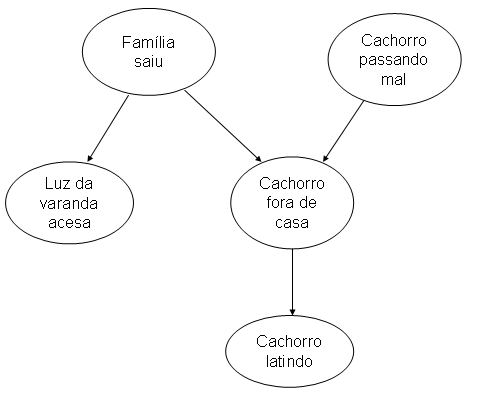
\includegraphics[width = 300px]{figuras/BN1}
	\caption[Exemplo family-out]{Exemplo family-out}
	\label{fig:familyBN}
\end{figure}

Nesse exemplo, suponhamos que se queira determinar se a família está em casa ou se ela saiu. Pelo grafo, podemos perceber que o fato de a luz da varanda estar acesa e de o cachorro estar fora de casa são indícios de que a família tenha saído. 

\section{Definição Formal}
Considere a \gls{bn} contendo $n$ nós, $X_1$ até $X_n$, tomados nesta ordem. Uma instanciação da distribuição disjunta de probabilidade é representada por $P(X_1 = x_1, X_2 = x_2, ... , X_n = x_n)$, ou de forma compacta $P(x_1, x_2, ..., x_n)$. A \textbf{regra da cadeia} nos permite fatorar probabilidades disjuntas como:
\begin{equation}
	P(x_1, x_2, ..., x_n) = P(x_1)P(x_2|x_1)...P(x_n|x_1,..,x_{n-1})\\
	= \prod_{i}^{}P(x_i|x_1,...,x_{i-1})
\end{equation}
No entanto, a estrutura de uma \gls{bn} implica que o valor de um nó em particular é condicionado apenas aos valores dos nós pais, o que reduz a equação acima à:
\begin{equation}\label{eq:pearl}
P(x_1, x_2, ..., x_n) = \prod_i P(x_i|pa_i)
\end{equation}
Onde $pa_i$ são os nós pais de $x_i$

\section{D-separation}
Segundo Cheng\cite{cheng02} Uma rede bayesiana pode ser vista como um sistema de rede de canais de informação, onde cada não é uma válvula que está aberta ou fechada e as válvulas são conectadas por canais de informação ruidosos (arestas). O fluxo de informação pode passar por um válvula aberta, mas não por uma válvula fechada. Quando todas as válvulas sobre um caminho entre dois não estão abertas, diz-se que este caminho é aberto. Se qualquer válvula no caminho está fechada, diz-se que o caminho é fechado.

Formalmente um caminho c é dito ser d-separado (ou bloqueado) por um conjunto de nós \textbf{Z} se e somente se:
\begin{itemize}
	\item c contem uma cadeia i $\rightarrow$ m $\rightarrow$ j ou uma divergência i $\leftarrow$ m $\rightarrow$ j tal que o nó do meio m está em \textbf{Z};
	\item c contem uma convergência (ou colisor) i $\rightarrow$ m $\leftarrow$ j tal que o nó do meio não está em $\textbf{Z}$ e nenhum descendente de m está em $\textbf{Z}$
\end{itemize}

O conjunto \textbf{Z} d-separa \textbf{X} de \textbf{Y} se e somente se, \textbf{Z} bloqueia todos os caminhos de nós em \textbf{X} para nós em \textbf{Y}.

Se um caminho satisfaz a condição acima, diz-se que ele é bloqueado; caso contrário ele é ativado por \textbf{Z}. Na figura \ref{fig:d-sep} $X$ = {2} e $Y$ = {3} são d-separados por Z = {1}; o caminho 2 $\leftarrow$ 1 $\rightarrow$ 3 é bloqueado por 1 $\in$ \textbf{Z}.
\begin{figure}[H]
	\centering
	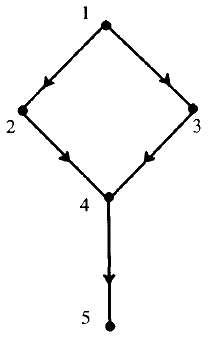
\includegraphics{figuras/d-separation}
	\caption[Exemplo D-separation]{Um \gls{dag} demostrando d-separation; o nó 1 bloqueia o caminho 2-1-3, enquanto o nó 5 ativa o caminho 2-4-3 (retirado de \cite{pearl88})}
	\label{fig:d-sep}
\end{figure}

Em 1988 Pearl prova que os conjuntos \textbf{X} e \textbf{Y} são d-separados por \textbf{Z} em \gls{dag} se e somente se \textbf{X} é independente de \textbf{Y} condicionado a \textbf{Z} em toda distribuição compatível com G.

Em outras palavras $(\textbf{X} \perp \textbf{Y}|\textbf{Z})_G \Leftrightarrow (\textbf{X}\perp\textbf{Y}|\textbf{Z})_P$, onde $(\textbf{X}\perp\textbf{Y}|\textbf{Z})_G$ significa que \textbf{X} é d-separado de \textbf{Y} dado \textbf{Z} em um grafo G, e $(\textbf{X}\perp \textbf{Y}|\textbf{Z})_P$ é a independência estatística como discutido na sessão anterior.

\section{M-separation}
Um teste alternativo para d-separação foi proposto por Lauritzen \cite{lauritzen90}, baseado na noção de grafos ancestrais e foi chamada de m-separação (separação moralizada) por Silva e Ladeira \cite{daSL02}.
\begin{itemize}
	\item Exclua de G todos os nós exceto aquele em anc(\textbf{X} $\cup$ \textbf{Y} $\cup$ \textbf{Z});
	\item Conecte por uma aresta todo par de nós que possuam filho em comum (moralização);
	\item Remova todas orientações dos arcos
\end{itemize}
Então $(\textbf{X} \perp \textbf{Y}|\textbf{Z})_G$ se e somente se, \textbf{Z} intercepta todos os caminhos entre \textbf{X} e \textbf{Y} no grafo não orientado resultante. Isto é, se removendo \textbf{X}, \textbf{Y} e \textbf{Z} ficam desconectados, então \textbf{X} e \textbf{Y}são condicionalmente independentes dado \textbf{Z}, caso contrário \textbf{X} e \textbf{Y} são dependentes dado Z. Onde \textbf(anc(W)) contém os nós de W e todos seus ancestrais.

O Benefício de m-separação sobre a d-separação é o fato de ser um processo algorítmico e portanto fácil de se implementar.

  % inserir demais capítulos
  

  \postextual
  \bibliographystyle{plain}
  \bibliography{bibliografia}

\appendix
  %\chapter{Documentação Original}%
\small\begin{verbatim}
% -*- mode: LaTeX; coding: utf-8; -*-
%%%%%%%%%%%%%%%%%%%%%%%%%%%%%%%%%%%%%%%%%%%%%%%%%%%%%%%%%%%%%%%%%%%%%%%%%%%%%%%
%% File    : unb-cic.cls (LaTeX2e class file)
%% Authors : Flávio Maico Vaz da Costa
%%              (based on previous versions by José Carlos L. Ralha)
%% Version : 0.93
%% Updates : 0.5  [??/11/2004] - Initial release. don't remember the day.
%%         : 0.75 [04/04/2005] - Fixed font problems, UnB logo
%%                               resolution, keywords and palavras-chave
%%                               hyphenation and generation problems,
%%                               and a few other problems.
%%         : 0.8  [08/01/2006] - Corrigido o problema causado por
%%                               bancas com quatro membros. O quarto
%%                               membro agora é OPCIONAL.
%%                               Foi criado um novo comando chamado
%%                               bibliografia. Esse comando tem dois
%%                               argumentos onde o primeiro especifica
%%                               o nome do arquivo de referencias
%%                               bibliograficas e o segundo argumento
%%                               especifica o formato. Como efeito
%%                               colateral, as referências aparecem no
%%                               sumário.
%%         : 0.9 [02/03/2008]  - Reformulação total, com nova estrutura
%%                               de opções, comandos e ambientes, adequação
%%                               do logo da UnB às normas da universidade,
%%                               inúmeras melhorias tipográficas,
%%                               aprimoramento da integração com hyperref,
%%                               melhor tratamento de erros nos comandos,
%%                               documentação e limpeza do código da classe.
%%         : 0.91 [10/05/2008] - Suporte ao XeLaTeX, aprimorado suporte para
%%                               glossaries.sty, novos comandos \capa, \CDU
%%                               e \subtitle, ajustes de margem para opções
%%                               hyperref/impressao.
%%         : 0.92 [26/05/2008] - Melhora do ambiente {definition}, suporte
%%                               a hypcap, novos comandos \fontelogo e
%%                               \slashedzero, suporte [10pt, 11pt, 12pt].
%%                               Corrigido bug de seções de apêndice quando
%%                               usando \hypersetup{bookmarksnumbered=true}.
%%         : 0.93 [09/06/2008] - Correção na contagem de páginas, valores
%%                               load e config para opção hyperref, comandos
%%                               \ifhyperref e \SetTableFigures, melhor
%%                               formatação do quadrado CIP. 
%%
%% Definição de classe para dissertações do departamento de
%% Ciência da Computação (CIC) da Universidade de Brasília.
%%
%%%%%%%%%%%%%%%%%%%%%%%%%%%%%%%%%%%%%%%%%%%%%%%%%%%%%%%%%%%%%%%%%%%%%%%%%%%%%%%
%% PRÉ-REQUISITOS (usando LaTeX ou XeLaTeX):
%%
%% * Uma distribuição LaTeX2e compatível
%%   - em Windows, recomenda-se MiKTeX: http://miktex.org/
%% * Logomarca da UnB (arquivos positivo_cor.eps e contorno_preto.eps)
%%   - disponível na página: http://www.unb.br/unb/marca/index.php
%% * Pacotes obrigatórios
%%   - xkeyval, graphicx, boites, setspace,
%%     geometry, atbegshi, hyperref
%%
%% PRÉ-REQUISITOS (usando XeLaTeX):
%% * Fonte "Arial" instalada no sistema operacional
%% * Pacotes obrigatórios
%%   - fontspec, xltxtra (carregar no próprio documento)
%%
%% PRÉ-REQUISITOS (usando LaTeX):
%% * Fonte ua1 (URW Arial A030, PostScript Type-1)
%%   - disponível no CTAN: http://www.ctan.org/tex-archive/fonts/urw/arial/
%%   - no MiKTeX, basta instalar pacote "arial" via MiKTeX Package Manager
%% * Pacotes obrigatórios
%%   - relsize, fixltx2e
%% * Pacotes opcionais
%%   - MinionPro (fonte proprietária)
%%
%%%%%%%%%%%%%%%%%%%%%%%%%%%%%%%%%%%%%%%%%%%%%%%%%%%%%%%%%%%%%%%%%%%%%%%%%%%%%%%
%% PRINCIPAIS OPÇÕES DISPONÍVEIS:
%%
%% licenciatura - O trabalho é do curso de Licenciatura (Graduação).
%% bacharelado  - O trabalho é do curso de Bacharelado (Graduação).
%% mestrado     - O trabalho é de Mestrado.
%%
%% draft - Gera o documento em modo de rascunho: não exibe as imagens e
%%         modifica o espaçamento entre linhas.
%% final - Gera o documento em modo final, não-rascunho (padrão).
%%
%% impressao       - Gera a versão para impressão, sem hipertexto.
%% hyperref=load   - Carrega e configura o pacote hyperref para gerar
%%                   a versão hipertexto para exibição em tela (padrão).
%% hyperref=config - Configura o pacote hyperref para gerar
%%                   a versão hipertexto para exibição em tela, mas o
%%                   pacote deve ser carregado no próprio documento.
%%                   Leia a seção PROBLEMAS CONHECIDOS para recomendação
%%                   de uso desta opção.
%%
%% 10pt - Define tamanho da fonte do texto.
%% 11pt - Define tamanho da fonte do texto (padrão no modo draft).
%% 12pt - Define tamanho da fonte do texto (padrão no modo final).
%%
%% singlespacing  - Define espaçamento simples entre linhas (padrão no modo
%%                  final).
%% onehalfspacing - Define espaçamento de um e meio entre linhas (padrão no
%%                  modo draft).
%% doublespacing  - Define espaçamento duplo entre linhas.
%% baselineskip   - Utiliza o comando \baselineskip para definir o espaçamento
%%                  de linhas. Se não for infomada, o espaçamento é definido 
%%                  pelo pacote "setspace" (recomendável, ou seja, só use esta
%%                  opção se tiver algum motivo para não usar o setspace).
%%                  Pode ser usada em conjunto com uma das três opções acima.
%%
%% prestyle=<val>  - Especifica o estilo das páginas iniciais (agradecimentos,
%%                   resumo, sumário, etc.). Valores típicos são "plain"
%%                   (padrão) ou "empty".
%% textstyle=<val> - Especifica o estilo das páginas dos elementos textuais e
%%                   pós-textuais. Valores típicos são "plain" (padrão) ou
%%                   "fancy" (este último requer o pacote {fancyhdr}).
%% chapstyle=<val> - Especifica o estilo da primeira página de cada capítulo.
%%                   Valores típicos são "plain" (padrão) ou "empty".
%%
%%%%%%%%%%%%%%%%%%%%%%%%%%%%%%%%%%%%%%%%%%%%%%%%%%%%%%%%%%%%%%%%%%%%%%%%%%%%%%%
%% CRIAÇÃO DA MONOGRAFIA:
%%
%% A folha de rosto e folha de aprovação, por padronização estética,
%% são sempre formatados como "onehalfspacing" independente das opções
%% escolhidas. A seção de Referências é sempre "singlespacing". Citações
%% {quote}, {quotation} e versos {verse} são automaticamente "singlespacing" e
%% com letra menor.
%%
%% Os comandos \textlinf (lining figures) e \texttabf (tabular figures)
%% permitem selecionar, respectivamente, números "maiúsculos" (sim, isso
%% existe!) e números monoespaçados - o que só faz sentido para fontes 
%% que conhenham números maiúsculos x minúsculos e monoespaçados x
%% proporcionais (Minion Pro, Myriad Pro, Didot, Apple Chancery...).
%% Essas opção foi implementada apenas para a fonte Adobe Minion Pro no LaTeX,
%% mas funciona para qualquer fonte que suporte este recurso no XeLaTeX -
%% veja a documentação do pacote {fontspec} para mais informações.
%% Use \textlinf quando os números acompanharem texto em letras maiúsculas ou
%% em versalete (small-caps). Use \texttabf em tabelas ou outros lugares onde
%% for desejável que os números fiquem alinhados em colunas. Como alternativa
%% aos comandos, pode-se usar os ambientes {linfig} e {tabfig}.
%% O comando \SetTableFigures pode ser usado para redefinir um ambiente de
%% modo que os números contidos nele sejam automaticamente formatados
%% maiúsculos e monoespaçados, por exemplo: 
%%
%%   \SetTableFigures{tabular}
%%   \SetTableFigures{tabularx}
%%   \SetTableFigures{longtable}
%%
%% A capa, quando presente, não é contada na numeração das páginas.
%% As páginas iniciais, a partir da folha de rosto, são consideradas na 
%% contagem de páginas, mas não são numeradas.
%% As páginas seguintes (lista de figuras, etc.) por padrão são numeradas com
%% algarismos romanos e aparecem no sumário. Entretanto, se prestyle=empty,
%% não recebem numeração nem aparecem no sumário. 
%% As páginas do conteúdo (da introdução em diante) são numeradas com 
%% algarismos arábicos (13, 14, 15...) e começam a partir de 1.
%%
%% O sumário, por razões óbvias, deve colocado antes de todas as páginas
%% que são mencionadas nele.
%%
%% O trabalho é dividido em elementos pré-textuais, textuais e pós-textuais.
%% Estes elementos (alguns são opcionais, converse com seu orientador)
%% são dispostos preferencialmente na seguinte ordem:
%%    ELEMENTO                COMANDOS MAIS IMPORTANTES
%%       Capa                 \capa
%%    Elementos pré-textuais  \pretextual
%%       Folha de rosto       \folharosto
%%       Ficha catalográfica  \cip (impressa no verso da folha de rosto)
%%       Errata               %deve ser criada como documento avulso
%%       Folha de aprovação   \folhaaprovacao
%%       Dedicatória          \begin{dedicatoria}...\end{dedicatoria}
%%       Agradecimentos       \begin{agradecimentos}...\end{agradecimentos}
%%       Epígrafe             %aluno-poeta, esse recurso não está disponível
%%       Resumo               \begin{resumo}...\end{resumo}
%%       Abstract             \begin{abstract}...\end{abstract}
%%       Lista de Figuras     \figuras
%%       Lista de Tabelas     \tabelas
%%       Lista de Siglas      \printglossary[type=acronym] %usando pacote {glossaries}
%%       Sumário              \sumario
%%    Elementos textuais      \textual
%%       Introdução           \chapter{Introdu\c{c}\~ao} ...
%%       Desenvolvimento      \chapter{Nome do capitulo} \section{Nome da secao} ...
%%       Conclusão            \chapter{Conclus\~ao} ...
%%    Elementos pós-textuais  \postextual
%%       Referências          \bibliographystyle{...} \bibliography %usar BibTeX
%%       Glossário            \printglossary %usando pacote {glossaries}
%%       Apêndices            \apendices \chapter{Nome do apendice} ...
%%       Anexos               \anexos \chapter{Nome do anexo} ...
%%       Índices              \printindex %usando pacote {makeidx}
%%
%% O comando \maketitle equivale a chamar:
%% \pretextual\folharosto\cip\folhaaprovacao
%%
%% A opção "impressao", além de ajustar as margens para melhor
%% encadernação, também faz \maketitle chamar internamente o
%% comando \capa.
%%
%% Caso esteja preparando a versão para visualização em tela
%% (hipertexto), o documento pode ser configurado com o comando
%% \hypersetup a ser chamado no preâmbulo - mais detalhes no
%% manual do pacote hyperref. Algumas opções interessantes,
%% com valores de exemplo, são:
%%   bookmarksnumbered=true,
%%	   (itens das seções exibidas no menu do PDF são numerados)
%%   linktocpage=true,
%%	   (links do sumário nos números de página, não nos nomes de seções)
%%   colorlinks=true,
%%	   (indica links pela cor do texto, não por retângulo ao redor)
%%   linkcolor=red!80!black,
%%	   (cor de links em geral, veja pacote xcolor para opções de cor)
%%   urlcolor=blue,
%%	   (cor de links para URLs - comando \url{http://...})
%%   citecolor=teal,
%%	   (cor de links para referências citadas no texto)
%%   pdfstartview=FitH
%%	   (PDF exibido inicialmente com zoom para largura da página)
%%
%% O comando \listas equivale a chamar:
%% \figuras\tabelas
%%
%% O alinhamento e formatação dos títulos é controlado pelos comandos
%% \pretextual, \textual e \postextual, de modo que em cada parte do trabalho
%% os títulos são apresentados de maneira diferente. Se quiser mudar o
%% alinhamento do título numa das partes do trabalho, logo após a chamada ao
%% comando acima, redefina o comando \chapteralign para aplicar o alinhamento
%% desejado. Se quiser fazer outras mudanças no formato (por exemplo, colocar
%% os títulos em versalete (small-caps), será necessário redefinir o comando
%% \chapterformat (veja exemplo no código da classe).
%%
%% Redefina o comando \fontelogo para mudar o nome da fonte a ser utilizada
%% no logo da UnB, sendo que o padrão é "Arial" (XeLaTeX) ou "ua1" (LaTeX).
%% Deve-se trocar por uma fonte parecida (como a Helvetica, "phv" no LaTeX)
%% apenas se não for possível a instalação da Arial.
%%
%% A classe adicionalmente provê o ambiente {definition}, que exibe
%% definições (conceituais) numeradas e formatadas com borda.
%%
%% Alguns dos comandos a serem chamados no preâmbulo (parte do código antes
%% da chamada a \begin{document}) são:
%% \title[] - Título do trabalho.
%% \subtitle[] - Subtítulo do trabalho (se houver).
%% \palavraschave[] - Lista de palavras-chave em português.
%% \keywords[] - Lista de palavras-chave em inglês.
%%   Os parâmetros opcionais definem como o valor será apresentado na página
%%   da CIP e nas propriedades do PDF, já que estas não podem conter macros
%%   (ex.: \title[Um estudo sobre PI elevado a PI]{Um estudo sobre $\pi^\pi$}).
%% \diamesano - Dia mês e ano.
%% \autor - Nome e sobrenome do autor.
%% \coautor - Nome e sobrenome do co-autor (se houver).
%% \coordenador[a] - Coordenador(a) do curso.
%% \orientador[a] - Orientador(a) do trabalho.
%% \coorientador[a] - Coorientador(a) do trabalho (se houver).
%% \membrobanca - Adiciona membros à banca (além do orientador e coorientador).
%% \CDU - Classificação Decimal Universal (por padrão é 004).
%%   Valores comuns para a área (conforme http://www.udcc.org/) são:
%%    004 Ciência da Computação e Tecnologia
%%    004.2	Arquitetura de computadores
%%    004.3	Hardware
%%    004.4	Software
%%    004.5	Interação homem-máquina
%%    004.6	Dados
%%    004.7	Comunicação de computadores
%%    004.8	Inteligência artificial
%%    004.9	Técnicas de informática orientadas a aplicação
%%
%%%%%%%%%%%%%%%%%%%%%%%%%%%%%%%%%%%%%%%%%%%%%%%%%%%%%%%%%%%%%%%%%%%%%%%%%%%%%%%
%% PROBLEMAS CONHECIDOS:
%%
%% * O pacote hyperref, embora muito útil para gerar um PDF para leitura em
%%   tela, tem inúmeros problemas de compatibilidade com outros pacotes -
%%   alguns só funcionam corretamente se forem carregados antes do hyperref.
%%   A opção [hyperref] (ou seu sinônimo [hyperref=load]) carregam o pacote
%%   na própria classe, o que impossibilita que algum pacote no documento do
%%   aluno seja carregado antes do hyperref. Neste caso, usar a opção
%%   [hyperref=config] junto com o comando \ifhyperref para carregar o
%%   hyperref apenas quando estiver sendo gerada uma versão para leitura em
%%   tela, como no seguinte exemplo:
%%
%%     %%% não carrega nameref com opção [impressao] 
%%     \ifhyperref{\usepackage{nameref}}{}
%%     %%% varioref só funciona se carregado entre nameref e hyperref
%%     \usepackage{varioref}
%%     %%% não carrega hyperref com opção [impressao] 
%%     \ifhyperref{\usepackage{hyperref}}{}
%%
%% * Recomenda-se o uso do XeTeX ou pdfTeX, já que o dvips (+ps2pdf)
%%   não suporta adequadamente links com quebra de linha. Quem deseja usar os
%%   recursos gráficos do PSTricks pode experimentar o pacote TikZ como
%%   alternativa que não depende de diretivas PostScript.
%% * O suporte para o modo matemático ainda não está completo no XeTeX. Se seu
%%   trabalho depende significativamente de fórmulas e equações, use o LaTeX
%%   (ou XeLaTeX com \usepackage[no-math]{fontspec} e uma fonte matemática do
%%   LaTeX que combine com a fonte escolhida para o texto).
%%
%%%%%%%%%%%%%%%%%%%%%%%%%%%%%%%%%%%%%%%%%%%%%%%%%%%%%%%%%%%%%%%%%%%%%%%%%%%%%%%
%% ORIENTAÇÕES TIPOGRÁFICAS:
%%
%% * Atenção aos diferentes tipos de traço:
%%      - O hífen (-) liga prefixos, sufixos, partículas e pronomes oblíquos
%%        (ex.: recordar-se, fazê-lo, co-habitar).
%%      - A meia-risca (--) indica intervalos numéricos e liga palavras
%%        independentes (ex.: páginas 1--5, viagem Londres--Estocolmo, São João
%%        del-Rei--MG).
%%      - O travessão (---) é usado em diálogos, quando o interlocutor muda,
%%        e pode substituir dois pontos, parênteses ou vírgulas em apostos.
%%   Antes e depois de travessão emprega-se espaço, nos demais casos não há 
%%   espaço.
%% * O ponto final marca o fim de uma sentença. Se o ponto for usado com outra
%%   finalidade, como numa abreviatura, usar \ (ou ~ se não quiser permitir 
%%   quebra de linha) para indicar ao TeX que não se trata de fim de sentença
%%   (ex.: Dr.\ Spock).
%% * Embora o padrão das normas ABNT (que, com suas "receitinhas de bolo", são
%%   bastante rudimentares quanto à tipografia) seja espaçamento duplo entre 
%%   linhas, o espaçamento deve ser escolhido de acordo com o tipo e tamanho
%%   das letras.
%%   A regra a ser seguida é: quanto maiores as linhas (quanto mais palavras
%%   por linha), maior deve ser o espaçamento entre elas. Muitas vezes o
%%   espaçamento simples é suficiente numa fonte bem elaborada, mas se o
%%   tamanho médio da linha for superior a 90 caracteres, pode-se aumentar a
%%   legibilidade definindo um modesto incremento de espaçamento (algo entre
%%   \SetSinglespace{1.1} e \SetSinglespace{1.15}).
%% * Como um trabalho acadêmico tem margens relativamente estreitas, para
%%   evitar que as linhas sejam muito longas, em modo final esta classe utiliza
%%   tamanho 12pt.
%%   Deve haver interesse nas opções 10pt ou 11pt apenas se estiver sendo
%%   utilizada uma fonte particularmente grande (por exemplo, que produza uma
%%   média inferior a 80 caracteres por linha a 12pt).
%% * Na tipografia brasileira e portuguesa é costume recuar (indentar) a
%%   primeira linha de cada parágrafo. Como esse recuo serve para destacar
%%   visualmente um parágrafo de seu anterior, o LaTeX não faz o recuo no
%%   primeiro parágrafo sob um título. Quem quiser indentar também o primeiro
%%   parágrafo só para "manter o costume" deve adicionar o pacote {indentfirst}
%%   ao seu documento.
%% * Citações com até três linhas ficam no próprio texto, marcadas por "aspas".
%%   Se o texto original contiver "aspas", trocá-las por 'aspas simples'.
%%   Se a citação tiver mais de três linhas e apenas um parágrafo, usar o
%%   ambiente {quote}. Se a citação tiver mais de um parágrafo, usar
%%   {quotation}. Nestes dois casos, não se deve circundar sua citação por
%%   aspas nem alterar as aspas do texto original.
%%   Se a citação começar com letra maiúscula, o texto imediatamente anterior
%%   deve terminar em dois pontos (:).
%% * Números ordinais em inglês são sucedidos por "st", "nd", "rd" ou "th",
%%   de acordo com o seguinte algoritmo:
%%      Se o número termina em 1 mas não termina em 11, use "st".
%%      Se o número termina em 2 mas não termina em 12, use "nd".
%%      Se o número termina em 3 mas não termina em 13, use "rd".
%%      Em quaisquer outros casos, use "th".
%%   Esse indicador de ordinal deve, preferencialmente, ser colocado como texto
%%   superscrito. Usar 112\textsuperscript{th} e não 112$^{th}$. Se não quiser
%%   se preocupar com essas regras, use o pacote {engord} com o comando
%%   \engordnumber{112}.
%% * Para indicar elipse (reticências), use \textellipsis,
%%   usar ... (ponto ponto ponto) não é a mesma coisa.
%%
%%%%%%%%%%%%%%%%%%%%%%%%%%%%%%%%%%%%%%%%%%%%%%%%%%%%%%%%%%%%%%%%%%%%%%%%%%%%%%%
%% FIM DA DOCUMENTAÇÃO
%%%%%%%%%%%%%%%%%%%%%%%%%%%%%%%%%%%%%%%%%%%%%%%%%%%%%%%%%%%%%%%%%%%%%%%%%%%%%%%
\end{verbatim}

\end{document}
